\section*{Einleitung}

Der Übergang von einem Bild in ein Anderes kann durch verschiedene
Effekte erreicht werden. Einer der bekanntesten ist die sogenannte
Kreuzblende (engl. cross dissolve). Dabei wird jeder Pixel des Quellbildes
sukzessive um $1-\frac{i}{numIterations}$ abgeschwächt und dafür jeder Pixel
des Zielbildes um $\frac{i}{numIterations}$ multipliziert (verstärkt). 
Das Resultat aus der Addition dieser beiden Operationen ergibt den
Effekt der eben genannten Kreuzblende (\ref{fig:dissolve}). Der Übergang
ist deutlich wahrnehmbar. Eine Verbesserung erreicht man durch die Verzerrung
beider Bilder in die Form des jeweilig anderen (\ref{fig:source} nach \ref{fig:dest} und umgekehrt).
Danach wird wie gehabt die Kreuzblende angewendet.
Die Resultierende Animation
kann den Eindruck erwecken als verwandle sich das Quell in das Zielbild.
Beier und Neely \cite{beierneely} entwickelten dafür einen Feature-basierten 
Algorithmus um diesen Effekt zu erzielen. Er kam in dem Michael Jackson Musikvideo
Black or White zum Einsatz \cite{cartoonbrew}. Die Testbilder, wie im folgenden Bericht zu sehen, sind aus jenem Musikvideo entwendet. \cite{blackorwhite}.
\begin{figure}[!htb]
	
	\centering
	\begin{subfigure}{0.4\textwidth}
		\centering
		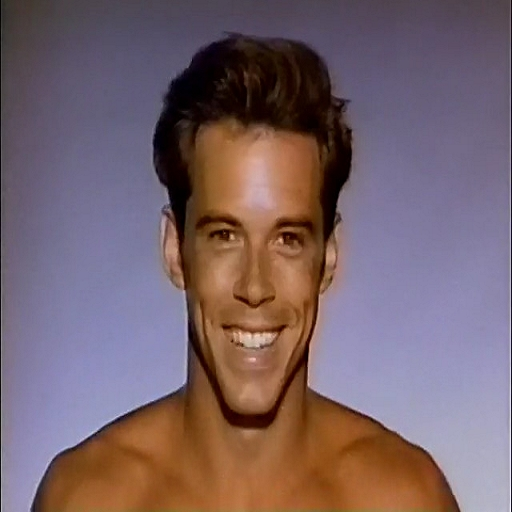
\includegraphics[width=\linewidth]{guy_squared.jpg}
		\caption{Quellbild}
		\label{fig:source}
	\end{subfigure}
	\hfill
	\begin{subfigure}{0.4\textwidth}
		\centering
		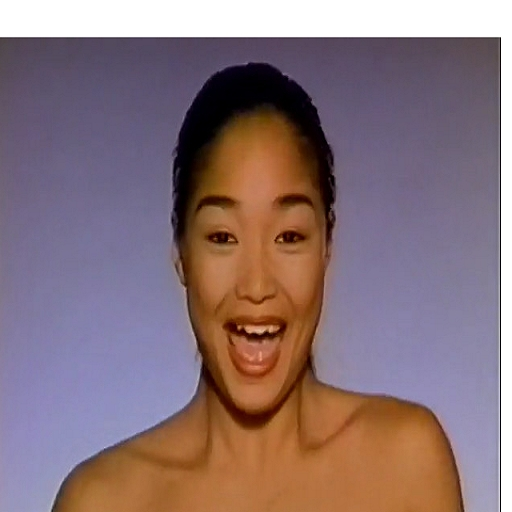
\includegraphics[width=\linewidth]{gal_squared.jpg}
		\caption{Zielbild}
		\label{fig:dest}
	\end{subfigure}
	
	\centering
	\begin{subfigure}{0.4\textwidth}
		\centering
		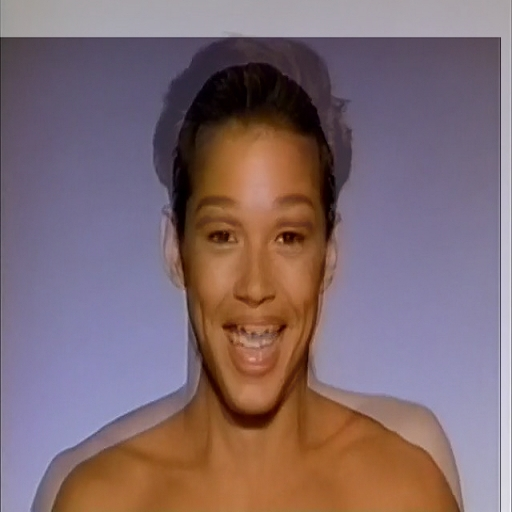
\includegraphics[width=\linewidth]{cross_dissolve_50pct.jpg}
		\caption{50\% Kreuzblende}
		\label{fig:dissolve}
	\end{subfigure}
	\hfill
	\begin{subfigure}{0.4\textwidth}
		\centering
		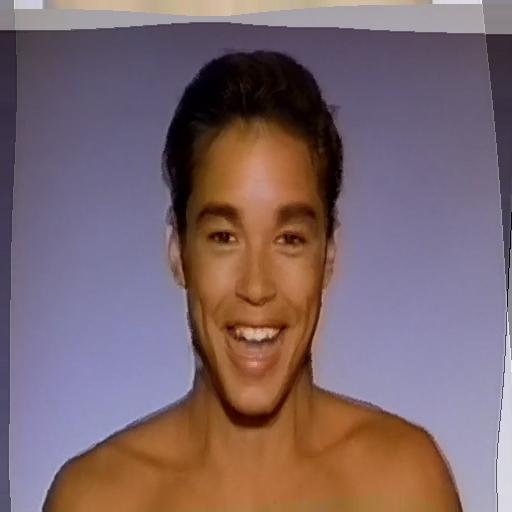
\includegraphics[width=\linewidth]{beierneely_50_pct.jpg}
		\caption{50\% Beier-Neely Morph}
		\label{fig:morph}
	\end{subfigure}
	\caption{Gegenüberstellung: einfache Kreuzblende und Beier-Neely Morphing}
	\label{fig:side-by-side}
	
\end{figure}
